\chapter{Binære Træer}
\label{ch:Binære Træer}

Træer som vi kender dem, har en stamme hvorfra grene springer ud. Fra grenene springer mindre grene, og på den måde ender træet med at have mange små grene, som stammer fra samme stamme, der ender hver sit sted. Binære træer er ikke langt fra denne forståelse af træer generelt: Binære træer har også en rod (eller stamme), hvorfra hele træet forgr\red{e}ner sig. Man tegner normalt binære træer som på figur \ref{fig:Eksempel på binært træ} bestående af knudepunkter og forbindelser mellem dem. Det specielle ved \emph{binære} træer, er at hvert knudepunkt højst må forgrene sig to gange (altså binært).

\section{Højden af et Binært Træ}
\label{sec:Højden af et Binært Træ}
Binære træers højde måles på hvor mange forgreninger, skal til for at nå det yderste blad.


\begin{figure}
	\begin{center}
		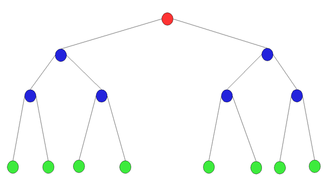
\includegraphics[scale=1]{../img/binary_tree.png}
	\end{center}
	\caption{Eksempel på binært træ. Træets balde er markeret med \green{grøn}, og roden med \red{rød}. \cite{binaert-trae}}
	\label{fig:Eksempel på binært træ}
\end{figure}

\section{Binære Træer og Sorteringsalgoritmer}
\label{sec:Binære Træer og Sorteringsalgoritmer}

Ved første blik kunne man tilgives for ikke, at se hvordan binære træer har relevans for sorteringsalgoritmer, men det kræver bare, at man giver knudepunkterne og grenene meningsfulde betydninger. I bund og grund er det som en sorteringsalgoritme gør, at fortage en masse sammenligninger af elementerne i dens input. Algoritmens bestemmer hvilke operationer, den skal køre udelukkede på baggrund af disse sammenligninger. Hvis vi tænker hvert knudepunkt som en sammenligning af to elementer fra algoritmens input (se figur \ref{fig:Binært Træ for Sammenligninger}), er det jo givet, at det ene element enten vil være større end det andet eller ikke. Denne sammenligning guider algoritmens operationer og derved den næste sammenligning. Dette gentages til algoritmen har gjort nok sammenligninger, til at kunne sortere dens input. Vi kan derfor tænke alle træets blade, som en måde for algoritmen at sortere et bestemt input; hvert blad har kun en vej til det, og vejen til bladet er udelukkede givet af algoritmens input, altså er hvert af træets blade en kollektion af de sammenligninger, som algoritmen gjorde for at sortere inputtet. 

\subsection{Det Mindste antal Sammenligninger}%
\label{sub:Det Mindste antal Sammenligninger}

I dette store teoretiske træ med alle dets blade kunne man jo så spørge: hvor mange sammenligninger skal der så højest til at sortere et input? eller omformuleret: hvor højt er træet? Denne oversættelse holder stik, da vi skal lave lige så mange sammenligninger for at komme ned til nederste blad, som træet er højt.

\begin{figure}
	\begin{center}
		\begin{tikzpicture}[scale = 1.5]
			\tikzstyle{comp} = [rectangle, draw, rounded corners];
			\node (12) at (0,0) {$e_1 \:?\: e_2$};
			\node (23) at (-3,-1)  {$e_2 \:?\: e_3$};
			\node (23b) at (3,-1)  {$e_2 \:?\: e_3$};
			\node (13) at (-2,-2)  {$e_1 \:?\: e_3$};
			\node (13b) at (2,-2)  {$e_1 \:?\: e_3$};
			\node (ww) at (-4,-2) {$e_1\leq e_2\leq e_3$};
			\node (1w3s2) at (-3,-3) {$e_1\leq e_3< e_3$};
			\node (3s1w2) at (-1,-3) {$e_3< e_1\leq e_2$};
			\node (2s1w3) at (1,-3) {$e_2< e_1\leq e_3$};
			\node (2w3s1) at (3,-3) {$e_2\leq e_3< e_1$};
			\node (1g2g3) at (4,-2) {$e_1> e_2> e_3$};
			\draw [->] (12) to node [above] {$\leq$} (23);
			\draw [->] (23) to node [above] {$\leq$} (ww);
			\draw [->] (12) to node [above] {$>$} (23b);
			\draw [->] (23) to node [above] {$>$} (13);
			\draw [->] (13) to node [above] {$\leq$} (1w3s2);
			\draw [->] (13) to node [above] {$>$} (3s1w2);
			\draw [->] (13b) to node [above] {$\leq$} (2s1w3);
			\draw [->] (13b) to node [above] {$>$} (2w3s1);
			\draw [->] (23b) to node [above] {$\leq$} (13b);
			\draw [->] (23b) to node [above] {$>$} (1g2g3);
		\end{tikzpicture}
	\end{center}
	\caption{Binært Træ. \cite[s. 109]{aogd}}
	\label{fig:Binært Træ for Sammenligninger}
\end{figure}

